\documentclass[submit,techrep,noauthor]{ipsj}

\usepackage[dvipdfmx]{graphicx}
\usepackage{latexsym}
\usepackage{amsmath,amssymb}

\newcommand{\Fcomp}{F_{\mathrm{comp}}}
\newcommand{\Rlaunch}{R_{\mathrm{launch}}}
\newcommand{\Rint}{R_{\mathrm{int}}}
\newcommand{\Nreq}{N_{\mathrm{req}}}
\newcommand{\Nsucc}{N_{\mathrm{succ}}}
\newcommand{\Nint}{N_{\mathrm{int}}}

\setcounter{巻数}{59}
\setcounter{号数}{1}
\setcounter{page}{1}


\begin{document}


\title{スポットインスタンスにおける実測に基づく\\実行条件決定モデルの構築}


\affiliate{DU}{同志社大学}

\author{那須 渚}{}{DU}[ctwn0144@mail4.doshisha.ac.jp]
\author{神野 敦哉}{}{DU}[ctwp0126@mail4.doshisha.ac.jp]
\author{田口 開智}{}{DU}[ctwp0168@mail4.doshisha.ac.jp]
\author{小比賀 亮仁}{}{DU}[akohiga@mail.doshisha.ac.jp]
\author{小板 隆浩}{}{DU}[tkoita@mail.doshisha.ac.jp]

\begin{abstract}
スポットインスタンスは，クラウド上の余剰計算資源を低価格で利用できる一方，
稼働中に中断される可能性がある．
中断による処理の再実行は，処理完了までの時間を延ばし，
計算資源の利用費用も増加させる．
既存研究ではSpot Placement Score（SPS）を用いた起動先の選択手法が検討されてきた．
しかしSPSは起動のしやすさを示す指標であり，
本研究の測定では，SPSが同じ値を示す状況でも起動後の中断率が時間帯によって異なっていた．
そこで本研究では，実測データに基づく実行条件選択モデルを提案する．
まず，所定の時間まで中断されずに稼働する割合を信頼性として定義し，
AWS上で2期間計15日間の測定を実施した．
その結果，信頼性はリージョン・インスタンスタイプ・時間帯によって異なる一方，
中断は稼働時間の経過によらずほぼ一定の確率で発生していた．
次に，再実行によって生じる時間的損失を「損失時間」と定義し，
その値を最小化する実行条件選択モデルを構築した．
実測データに基づくシミュレーションにより，
実行開始時刻の選択によって損失時間を33\%削減できることを確認した．
\end{abstract}


\begin{jkeyword}
スポットインスタンス，クラウドコンピューティング，中断，実行条件選択，損失時間
\end{jkeyword}



\maketitle

%1
\section{背景}
\label{sec:background}

クラウドコンピューティングの普及に伴い，
計算資源の利用コストは多くの利用者にとって重要な課題となっている．
コストを削減する手段の一つにスポットインスタンスがある\cite{AWSSpot}．
スポットインスタンスは，クラウドプロバイダの余剰計算資源を低価格で提供する料金モデルであり，
オンデマンドインスタンスと比較して最大約90\%の割引価格で利用できる\cite{Lin2022Survey}．
この価格優位性から，機械学習やバッチ処理に加え，
CI/CDにおける自動ビルドやテストのように
一時的に計算資源を必要とするワークロードにも利用されている\cite{Ramesh2025}．

\subsection{スポットインスタンスの中断}

スポットインスタンスは余剰容量に基づいて提供されるため，
利用者の都合とは無関係に中断されうる．
需要の増加や利用可能な容量の減少が生じると，
プロバイダは稼働中のインスタンスを回収する．
本稿ではこれを中断と呼ぶ．
AWSでは中断の約2分前に，
警告がAmazon EventBridgeのイベントおよびインスタンスメタデータとして通知される\cite{AWSInterruptNotice}．
ただしこの通知はベストエフォートで提供されるものであり，
また2分間で可能な対処は限られる．

中断は利用者に次の困難をもたらす．

\begin{itemize}
\item \textbf{再実行による損失}：
チェックポイントを取得していない場合，中断までの処理内容は失われ，
ワークロード全体の再実行が必要となる．
その結果，処理完了までの時間と利用費用がともに増加する．
\item \textbf{予測の困難さ}：
中断がいつ発生するかを利用者が事前に知ることはできない．
\item \textbf{条件による変動}：
中断のされやすさはリージョン，インスタンスタイプ，時間帯などによって
異なると考えられるが，
利用者がこの変動を把握する手段は限られている．
\end{itemize}

これらの困難は，CI/CDのビルドやテスト，短時間のバッチ処理のような
短時間ワークロードにおいて特に問題となる．
こうしたワークロードは実行時間こそ短いものの，
完了前に中断されればジョブ全体をやり直す必要があり，
中断のたびに実行時間と費用が積み重なる．
したがって利用者にとって重要なのは，
どのリージョン，インスタンスタイプ，実行時刻で実行すれば
処理を中断されずに完了できるかという判断である．
本稿では，これらの組合せを\textbf{実行条件}と呼ぶ．

\subsection{Spot Placement Score}

この判断を支援する指標として，AWSはSpot Placement Score（SPS）を提供している\cite{AWSSPS}．
SPSは，指定したインスタンスタイプ，リージョン，必要容量の条件下で
スポットリクエストが成立する見込みを1から10のスコアで示す指標である．
スコアが高いほど，要求した容量を確保できる見込みが高い．
SPSはリージョン単位またはアベイラビリティゾーン単位で取得できる．
既存研究では，SPSを用いて起動先やマイグレーション先を選択する手法が検討されてきた\cite{Katayama2022}．

しかしSPSが対象とするのはリクエスト時点での容量の確保，すなわち起動のしやすさであり，
起動したインスタンスが必要な処理時間だけ中断されずに稼働し続けられるかは対象としていない．
短時間ワークロードの利用者にとって，
起動に成功することと処理が完了することは別の問題である．
本研究ではこの違いを，
\textbf{起動のしやすさ}と\textbf{起動後の継続性}の区別として扱う．

\subsection{本研究の目的}

以上を踏まえ，本研究では，プロバイダ固有の指標に依存せず，
自ら測定した起動・中断の記録のみに基づいて実行条件を選択するモデルを提案する．
本稿の貢献は次の3点である．

\begin{itemize}
\item 起動の成否と起動後の中断を分離して記録する測定フレームワークを実装し，
所定の期限まで中断されずに稼働する割合を
期限条件付き完了可能性として定義した．
\item AWSの4リージョン・3インスタンスタイプを対象とした
2期間計15日間の測定（起動リクエスト4,320件）により，
期限60分の完了可能性が実行条件によって0.73から1.00まで変動すること，
および中断ハザード率が稼働時間の経過に対して増加しないことを示した．
\item 再実行による時間的損失を損失時間として定式化し，
入力がすべて実測値である実行条件選択モデルを構築した．
測定データを用いたシミュレーションにより，
実行開始時刻の選択によって損失時間が33\%削減されることを示した．
\end{itemize}

以降，\ref{sec:related}章で関連研究を整理し，
\ref{sec:prelim}章でSPSと起動後の継続性の関係を測定データにより確認する．
\ref{sec:measure}章で信頼性の指標と測定方法を，
\ref{sec:result}章で測定結果を示す．
\ref{sec:model}章で実行条件選択モデルを構築し，
\ref{sec:eval}章で評価する．
\ref{sec:discussion}章で考察と本研究の限界を述べ，
\ref{sec:conclusion}章でまとめる．


%2
\section{関連研究}
\label{sec:related}

\subsection{スポットインスタンスの可用性向上}

Linら\cite{Lin2022Survey}はスポットインスタンスの可用性を向上させる手法を調査し，
チェックポイント，マイグレーション，レプリケーション，スケジューリングといった
アプローチに整理している．
本研究が扱う実行条件の選択はスケジューリングに相当する．
また\ref{sec:checkpoint}節で比較する定期的なジョブの分割は，
チェックポイントに相当する．

\subsection{プロバイダの指標に基づく選択}

Katayamaら\cite{Katayama2022}は，
中断発生時のマイグレーション先として
SPSがより高いリージョンまたはアベイラビリティゾーンを選択する手法を提案し，
再起動の成功率を高められることを示した．
またGargら\cite{Garg2025}は，
スポット価格の変動を考慮した入札戦略によりクラウド費用を削減する手法を検討している．
これらの手法は起動時点の可用性や費用の観点からは有効であるが，
起動したインスタンスがワークロードの完了まで稼働し続けられるかは，
これらの指標からは直接判断できない．

\subsection{中断挙動の観測}

Kimら\cite{Kim2024SpotInterruption}は，
SPSが時間帯や曜日に応じて周期的に変動すること，
およびSPSとスポットインスタンスの生存時間との間に一定の関係があることを示している．
Leeら\cite{Lee2022SpotLake}は，SPS，スポット価格，中断率などを継続的に収集する
アーカイブサービスSpotLakeを提案し，
GPUインスタンスや大規模なインスタンスタイプで可用性が低い傾向を報告している．
これらの研究は中断挙動の統計的性質を明らかにしているが，
観測された変動は主に記述・分析の対象として扱われており，
実行条件を選択するための入力として用いる枠組みは十分に検討されていない．

本研究は，プロバイダ固有の指標ではなく自ら測定した中断の記録を用い，
それを実行条件の決定に直接用いる点でこれらの研究と異なる．


%3
\section{SPSと起動後の継続性}
\label{sec:prelim}

\ref{sec:background}章で述べたとおり，SPSは起動のしやすさを示す指標として提供されている．
一方，Kimら\cite{Kim2024SpotInterruption}はSPSと生存時間の間に一定の関係があることを報告している．
そこで本章では，SPSを用いて中断されにくい実行条件を選べるかを，本研究の測定データにより確認する．

\subsection{方法}

\ref{sec:measure}章で述べる測定のうち，
SPSを記録した2026年10月10日から18日までの8日間（192時間）のデータを用いる．
対象は4リージョン・3インスタンスタイプである．
起動リクエストは2,304件，起動成功は2,114件であり，
このうち124件が起動から60分以内に中断された．
SPSには，リクエスト時に記録した値を用いる．
以下では，起動したインスタンスが期限$d$まで中断されずに稼働した割合を
$\Fcomp(d)$と書く（\ref{sec:measure}章で定義する）．

観測されたSPSは，インスタンスタイプごとにほぼ一定の値をとった．
c6a.largeでは90\%が3，g4dn.xlargeでは57\%が9であり，
それ以外の大部分は1であった．
そこで各タイプで最も多く観測された値を通常値とし，
SPSが通常値を下回った場合を\textbf{SPS低下}とする．
t3.microはSPSがほぼ常に3であり，中断も1件のみであったため，分析から除く．

\subsection{SPSの低下と中断}

SPS低下時の$\Fcomp(60)$は，c6a.largeで0.72（95\%信頼区間0.60--0.81，$n=67$），
g4dn.xlargeで0.69（0.61--0.76，$n=158$）であり，
SPSが通常値のとき（いずれも0.95）より低かった．
リージョンとインスタンスタイプで層別したMantel-Haenszel推定によると，
SPS低下時に60分以内に中断されるオッズは通常時の約7.0倍（95\%信頼区間4.5--10.8）であった．
したがって，SPSは起動後の中断と無関係ではなく，
この結果はKimら\cite{Kim2024SpotInterruption}の報告と整合する．

ただし，SPSの低下は個々の起動の中断を予測するものではない．
SPS低下時に起動したインスタンスの70\%は60分間中断されず，
一方で分析対象の中断123件のうち55件（45\%）はSPSが通常値のときに発生した．
また，起動成功の大部分（c6a.largeで91\%，g4dn.xlargeで73\%）は
SPSが通常値のときに起動しており，
このときSPSは実行条件の間に差をつけない．

\subsection{同じSPSのもとでの継続性の差}

\begin{table}[tb]
\caption{SPSが通常値（3）のときの時間帯別の$\Fcomp(60)$
（c6a.large，4リージョン合計）}
\label{tab:prelim}
\centering
\begin{tabular}{lrcr}\hline\hline
時間帯 & $\Fcomp(60)$ & 95\%信頼区間 & $n$\\\hline
Night     & 0.99 & 0.96--1.00 & 190\\
Morning   & 0.92 & 0.87--0.95 & 162\\
Afternoon & 0.92 & 0.87--0.95 & 152\\
Evening   & 0.97 & 0.94--0.99 & 184\\\hline
\end{tabular}
\end{table}

SPSでは区別できない継続性の差があるかを調べるため，
SPSが通常値のときの起動に限って$\Fcomp(60)$を時間帯別に求めた．
\tabref{tab:prelim}に示すように，c6a.largeでは
SPSがすべて3であるにもかかわらず，$\Fcomp(60)$はNightの0.99に対し
MorningとAfternoonでは0.92であった．
中断率に換算するとNightの1.1\%に対しMorningは8.0\%であり，
95\%信頼区間は重ならない（時間帯間の差の$\chi^2$検定，$p=0.002$）．
なお，g4dn.xlargeでは同様の差は有意ではなかった（$p=0.43$）．
また，両タイプを合わせ，SPS低下，リージョン，インスタンスタイプを説明変数とする
ロジスティック回帰に時間帯を加えると，
当てはまりは有意に改善した（尤度比検定，$p<0.001$）．
すなわち，時間帯による中断されやすさの差の一部はSPSに現れない．

\subsection{まとめ}

以上より，SPSは中断と無関係ではないものの，
SPSが同じ値を示す状況での継続性の差を区別することはできない．
時間帯による差にはSPSに現れない成分が含まれるため，
SPSのみに基づく選択ではこの差を利用できない．
また，SPSの通常値はインスタンスタイプによって異なり（c6a.largeでは3，g4dn.xlargeでは9），
両者の$\Fcomp(60)$は同程度であったことから，
SPSの値はタイプ間の比較にも用いることができない．
中断されにくい実行条件を選ぶには，
実行条件ごとの完了可能性を実測に基づいて求める必要がある．


%4
\section{期限条件付き完了可能性の測定}
\label{sec:measure}

\subsection{指標の定義}

本研究では，短時間ワークロードの信頼性を，
起動したインスタンスが所定の期限まで中断されずに稼働する割合として定義する．
測定では実際のアプリケーションは実行せず，
期限$d$まで中断されずに稼働し続けたことをもって，
処理時間が$d$以下のワークロードが完了可能であったとみなす．

起動リクエスト数を$\Nreq$，起動に成功したインスタンス数を$\Nsucc$，
起動に成功したインスタンスのうち期限$d$より前に中断された数を$\Nint(d)$とする．
起動成功率$\Rlaunch$と期限前中断率$\Rint(d)$を次のように定義する．
\begin{equation}
\Rlaunch = \frac{\Nsucc}{\Nreq}, \qquad
\Rint(d) = \frac{\Nint(d)}{\Nsucc}
\end{equation}
そのうえで，\textbf{期限条件付き完了可能性}$\Fcomp(d)$を次式で定義する．
\begin{equation}
\Fcomp(d) = 1 - \Rint(d)
\label{eq:fcomp}
\end{equation}

$\Rlaunch$と$\Fcomp(d)$を分けて定義することで，
起動時点の可用性と起動後の継続性を区別して扱える．
SPSが対象とするのは前者であり，$\Fcomp(d)$が対象とするのは後者である．
両者は排他的ではなく，信頼性の異なる側面を捉える相補的な指標である．

\subsection{測定フレームワーク}
\label{sec:framework}

\begin{figure}[tb]
\centering
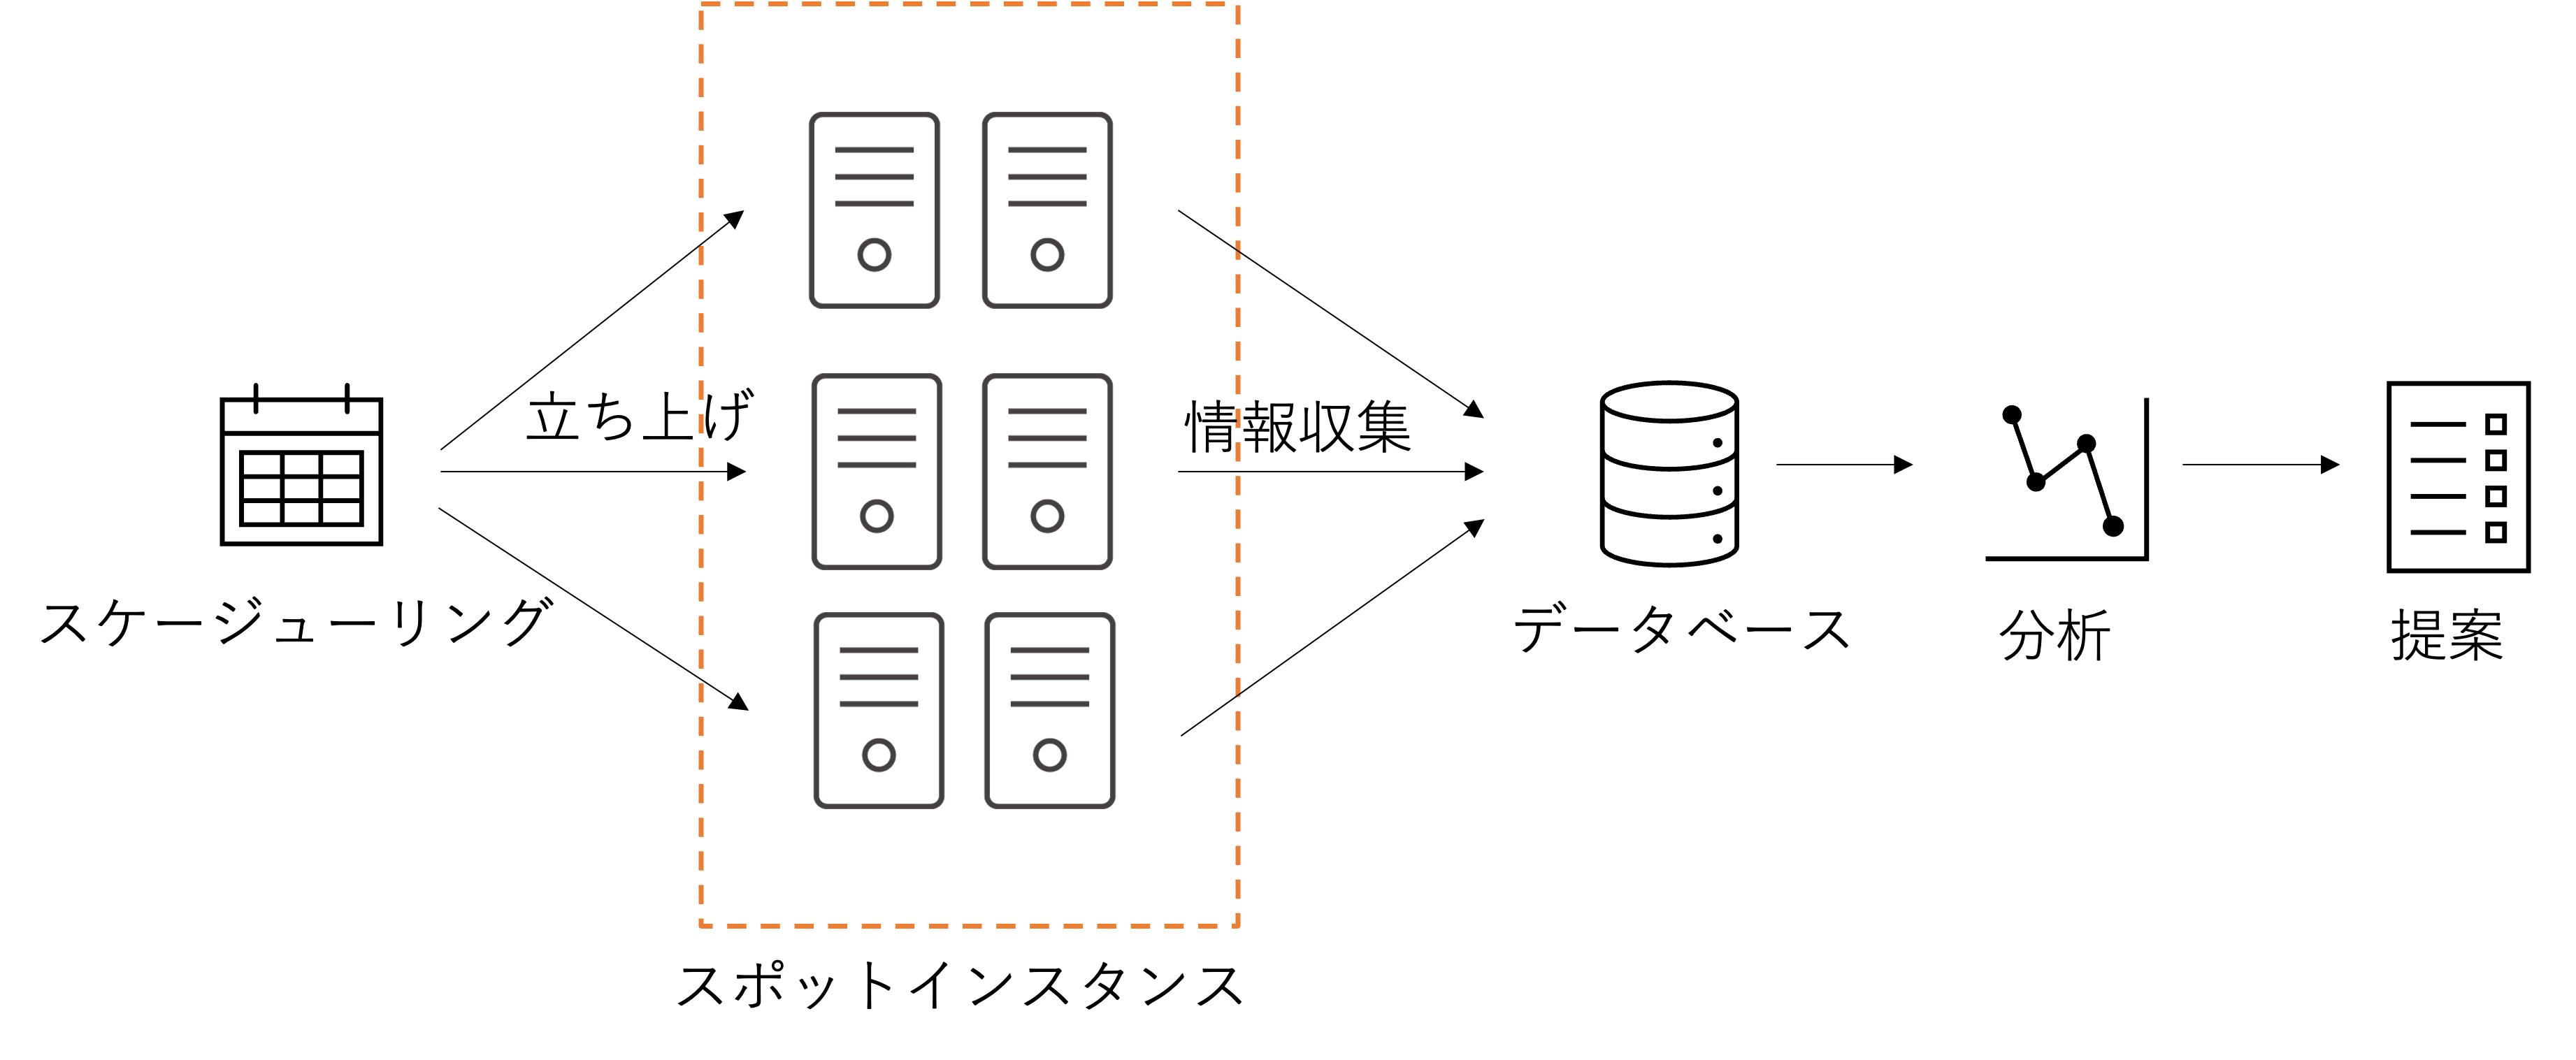
\includegraphics[width=\columnwidth]{figures/artect.png}
\caption{測定フレームワークの概要}
\label{fig:framework}
\end{figure}

\figref{fig:framework}に測定フレームワークの概要を示す．
本フレームワークはTerraformにより各リージョンに同一の構成で構築し，
AWS Lambda，Amazon EventBridge，Amazon DynamoDBを用いて実装した．

EventBridgeのスケジュールにより起動用のLambda関数を毎時0分に実行し，
対象の各インスタンスタイプについてスポットインスタンスを1台ずつ要求する．
容量不足などアベイラビリティゾーン単位のエラーでリクエストが失敗した場合は，
同一リージョン内の別のゾーンで再試行し，
いずれのゾーンでも成立しなかった場合を起動失敗とする．
リクエスト時には対象ゾーンのスポット価格を記録し，10月の測定ではSPSもあわせて記録した．

起動したインスタンスは1時間の観測期間にわたって稼働し，
期間が終了するとインスタンス自身が停止して終了する．
中断の検知には二つの経路を用いる．
一つはインスタンス内部で5秒ごとにインスタンスメタデータを確認する経路であり，
もう一つはEventBridgeが通知する中断警告イベントをLambda関数で受け取る経路である．
いずれかの経路で中断警告を検知したインスタンスを中断として記録し，
起動からの経過時間をあわせて記録する．
また，インスタンスの状態遷移イベントから
起動時刻，running状態への遷移時刻，配置されたゾーンを記録する．
これらの記録はすべてDynamoDBに集約する．

\subsection{実験設定}

\begin{table}[tb]
\caption{対象インスタンスタイプ（価格は観測期間中の4リージョン平均スポット価格）}
\label{tab:specs}
\centering
\begin{tabular}{llr}\hline\hline
タイプ & 分類 & 価格 (USD/h)\\\hline
c6a.large   & 計算最適化     & 0.039\\
g4dn.xlarge & GPU（T4）搭載  & 0.307\\
t3.micro    & バースト可能   & 0.005\\\hline
\end{tabular}
\end{table}

対象のインスタンスタイプは，リソース特性の異なる
c6a.large，g4dn.xlarge，t3.microの3種類とした\cite{Pham2018,AWSInstanceTypes}
（\tabref{tab:specs}）．
対象リージョンは，N.~Virginia（us-east-1），Ireland（eu-west-1），
Tokyo（ap-northeast-1），Singapore（ap-southeast-1）の4つである．
各リージョンで各インスタンスタイプを1時間に1台起動し，
2026年5月19日から25日までの7日間と，
10月10日から18日までの8日間（192時間）の計15日間測定した．
最大スポット価格は指定していない．

時間帯の影響を分析するため，各リージョンのローカル時刻に基づいて1日を
Night（0--6時），Morning（6--12時），Afternoon（12--18時），Evening（18--24時）の
4区間に分割した．
リージョン，インスタンスタイプ，時間帯の組合せは48通りであり，
各組合せにつき90件（6時間$\times$15日）の起動リクエストを送信した．


%5
\section{測定結果}
\label{sec:result}

\subsection{全体の傾向}

測定期間中に$\Nreq=4{,}320$件の起動リクエストを送信し，
このうち$\Nsucc=4{,}064$件が起動に成功した（$\Rlaunch=94.1\%$）．
起動に成功したインスタンスのうち251件（6.2\%）が，
1時間の観測期間の終了前に中断された．
全データをまとめた$\Fcomp(d)$は，
$d=5$，10，30，60分に対してそれぞれ0.994，0.988，0.967，0.943であった．
また，起動リクエストからインスタンスがrunning状態となるまでの
起動オーバーヘッドは，平均4.42秒（中央値4秒，最大31秒）であった．

\subsection{実行条件による変動}
\label{sec:variation}

\begin{figure*}[t]
\centering
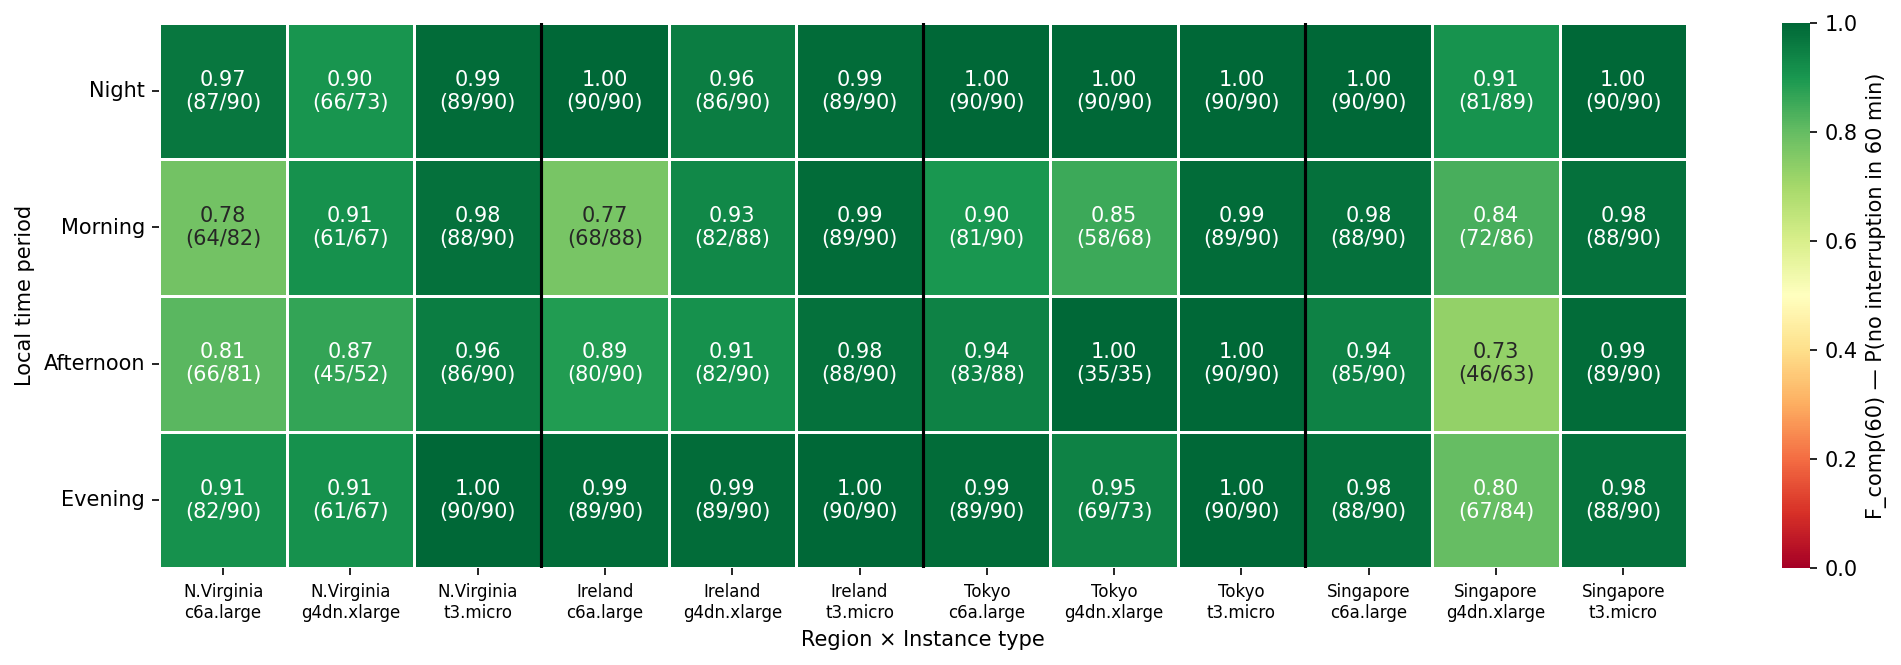
\includegraphics[width=\textwidth]{figures/figure1_fcomp60_heatmap.png}
\caption{リージョン，インスタンスタイプ，時間帯別の$\Fcomp(60)$．
括弧内は（60分間中断されなかった数/起動成功数）を示す．}
\label{fig:heatmap}
\end{figure*}

\figref{fig:heatmap}に，リージョン，インスタンスタイプ，時間帯ごとの$\Fcomp(60)$を示す．
t3.microはすべての条件で$\Fcomp(60)\geq 0.96$であり，中断の影響を受けにくかった．
一方，c6a.largeとg4dn.xlargeでは条件による変動が大きく，
$\Fcomp(60)$は0.73から1.00の範囲で変化した．

\begin{table}[tb]
\caption{N.~Virginia，c6a.largeにおける時間帯別の$\Fcomp(60)$}
\label{tab:nv}
\centering
\begin{tabular}{lrcr}\hline\hline
時間帯 & $\Fcomp(60)$ & 95\%信頼区間 & $n$\\\hline
Night     & 0.97 & 0.91--0.99 & 90\\
Morning   & 0.78 & 0.68--0.86 & 82\\
Afternoon & 0.81 & 0.72--0.88 & 81\\
Evening   & 0.91 & 0.83--0.95 & 90\\\hline
\end{tabular}
\end{table}

最も大きな変動は，N.~Virginiaのc6a.largeで観測された（\tabref{tab:nv}）．
NightとMorningの差は約0.19であり，
Wilsonの95\%信頼区間\cite{Wilson1927}は重ならない．
したがって，この差が標本変動のみによって生じた可能性は低い．

また，$\Fcomp(60)$が最も低くなる時間帯はリージョンによって異なっていた．
N.~VirginiaとIrelandのc6a.largeではMorningが最も低く，
Singaporeのg4dn.xlargeではAfternoonが最も低かった．
この傾向は，中断が各地域のクラウド需要の日内変動に対応しているという解釈と整合する．

\subsection{中断ハザード率}
\label{sec:hazard}

\begin{figure}[tb]
\centering
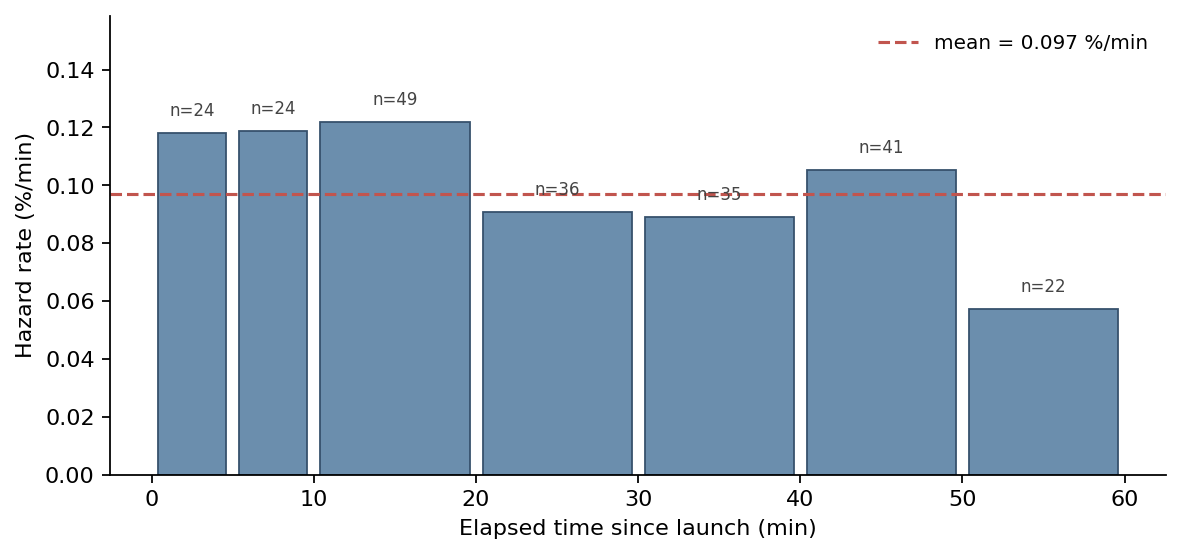
\includegraphics[width=\columnwidth]{figures/figure3_hazard.png}
\caption{経過時間別の中断ハザード率．
破線は平均値，$n$は各区間の中断件数を示す．}
\label{fig:hazard}
\end{figure}

中断が稼働時間の経過に対してどのように発生するかを調べるため，
経過時間の区間ごとに，区間の開始時点で稼働していたインスタンス数で
中断件数を正規化したハザード率を求めた（\figref{fig:hazard}）．
ハザード率は0.057--0.122\%/分の範囲で変動したが，
経過時間に対して単調に増加する傾向は見られなかった．
すなわち，長く稼働したインスタンスほど中断されやすくなるという性質は観測されず，
中断は単位時間あたりほぼ一定の確率で発生する事象として振る舞った．

\ref{sec:variation}節の結果と合わせると，
中断のされやすさは稼働時間の長さよりも実行条件によって決まると考えられる．
ただし，60分以内の中断231件という標本数ではハザード率が一定であることを
統計的に強く主張することはできない．
本稿では，単調増加を示す証拠は得られなかったという主張にとどめる．


%6
\section{実行条件選択モデル}
\label{sec:model}

\subsection{損失時間}

中断されたジョブは再実行されるため，
利用者が要する総時間は本来の処理時間を上回る．
本稿ではこの超過分を\textbf{損失時間}と呼び，モデルの最小化対象とする．
損失時間は，やり直す回数と，1回あたりの中断までに費やした時間の積として表される．
前者は実行条件の中断されにくさによって決まり，
後者は中断が発生するまでの経過時間によって決まる．

ジョブは時刻$t_0$に到着し，処理時間$d$を持つとする．
また開始時刻を最大$\Delta$だけ遅らせてよいとし，$\Delta$を許容遅延と呼ぶ．
決定変数は，リージョン$r$，インスタンスタイプ$\tau$，実行開始時刻$t$である．
時刻$t$におけるリージョン$r$のローカル時間帯を$\pi=\pi(r,t)$と書く．

実行条件$(r,\tau,\pi)$のもとで処理が完了する確率$p$は，
式(\ref{eq:fcomp})の期限条件付き完了可能性そのものである．
\begin{equation}
p(r,\tau,\pi,d) = \Fcomp^{(r,\tau,\pi)}(d)
\end{equation}
各試行が独立であると仮定すると，
成功するまでの試行回数は幾何分布に従い，その期待値は$1/p$である．
したがって，やり直す回数の期待値は$1/p-1$となる．
また，中断された試行で費やされた時間の期待値を
\begin{equation}
\bar{u}(r,\tau,\pi,d) = \mathrm{E}\left[\,U \mid U<d\,\right]
\end{equation}
とする．ここで$U$は起動から中断までの稼働時間である．
以上より，損失時間$L$を次式で定義する．
\begin{equation}
L(r,\tau,t) = \left(\frac{1}{p(r,\tau,\pi,d)}-1\right)\bar{u}(r,\tau,\pi,d) + s
\label{eq:loss}
\end{equation}
ここで$s$は起動オーバーヘッドである．
$p$，$\bar{u}$，$s$はいずれも\ref{sec:result}章の測定データから直接算出でき，
プロバイダ固有の指標を必要としない．

\subsection{設計上の判断}

\textbf{最小化対象．}
最小化対象として利用料金も考えられるが，本研究では損失時間を用いる．
料金を目的関数とすると，リージョン間の価格差が中断特性の差を覆い隠すためである．
たとえばc6a.largeの観測スポット価格は，
N.~Virginiaの0.0301 USD/hに対しTokyoでは0.0445 USD/hと48\%高い．
一方，中断による課金時間の増加は数パーセントにとどまる．
このため料金を最小化すると，中断特性によらず常に最安のリージョンが選ばれる．

\textbf{推定誤差への対処．}
完了確率$p$は，条件あたり高々90件の標本から推定した値である．
最適化は最も良く見える条件を選ぶため，
点推定値をそのまま用いると偶然良好な値を示した条件を選びやすい．
そこで条件の選択には，$p$の代わりに
Wilsonの95\%下側信頼限界$\tilde{p}$\cite{Wilson1927}を用いる．
$\tilde{p}$は標本数が少ないほど点推定値から大きく下がるため，
標本の少ない条件は選ばれにくくなる．
なお，効果の評価には点推定値$p$を用いる．

\subsection{最適化問題}

実行条件の選択は，次の最適化問題として記述される．
\begin{equation}
\begin{aligned}
\min_{r,\,\tau,\,t}\quad & L(r,\tau,t)\\
\mathrm{s.t.}\quad
 & t_0 \leq t \leq t_0 + \Delta\\
 & r\in\mathcal{R},\quad \tau\in\mathcal{T}\\
 & p(r,\tau,\pi(r,t),d) \geq p_{\min}
\end{aligned}
\label{eq:opt}
\end{equation}
$\mathcal{R}$，$\mathcal{T}$は利用可能なリージョンとインスタンスタイプの集合，
$p_{\min}$は利用者が求める完了確率の下限である．
$\Delta=0$のとき$t=t_0$となり，選択できるのはリージョンとインスタンスタイプのみとなる．
実行開始時刻を1時間単位で選ぶ場合，
候補は高々$4\times3\times24=288$通りであり，全列挙により厳密に解ける．

\subsection{決定手続き}
\label{sec:procedure}

式(\ref{eq:opt})は次の2段階で解く．
第1段階（オフライン）では，測定データから実行条件ごとの
$p$，$\tilde{p}$，$\bar{u}$を算出し，表として保持する．
条件数は48であり，表は小さい．
第2段階（オンライン）では，ジョブの到着時に許容遅延の範囲で候補を列挙し，
損失時間が最小となる条件を選ぶ．

\begin{table}[tb]
\caption{到着時刻ごとの決定例（N.~Virginia，c6a.large，$d=60$分，$\Delta=6$時間）．
到着時刻はUTC，$L$の単位は分，遅延の単位は時間．}
\label{tab:decision}
\centering
\setlength{\tabcolsep}{4pt}
\begin{tabular}{rlrrlr}\hline\hline
到着 & 時間帯 & $L$（即時） & 遅延 & 実行時間帯 & $L$（決定後）\\\hline
0時  & Evening   & 3.21 & 4 & Night     & 1.31\\
4時  & Night     & 1.31 & 0 & Night     & 1.31\\
10時 & Morning   & 6.65 & 6 & Afternoon & 5.07\\
16時 & Afternoon & 5.07 & 6 & Evening   & 3.21\\
22時 & Evening   & 3.21 & 6 & Night     & 1.31\\\hline
\multicolumn{2}{l}{24時刻の平均} & 4.06 & 2.6 & & 2.73\\\hline
\end{tabular}
\end{table}

\tabref{tab:decision}に，リージョンとインスタンスタイプを固定し
実行開始時刻のみを選択する場合の決定例を示す．
この例から次の3点が確認できる．
第一に，常に遅延させるわけではない．
24時刻のうち6時刻では遅延なしで実行される．
第二に，必ずしも最良の時間帯を選ぶわけではない．
10時に到着した場合，最良であるNightには許容遅延6時間では到達できないため，
到達可能な範囲で最良のAfternoonを選ぶ．
第三に，平均遅延は2.6時間であり，許容遅延の上限まで待つ必要は必ずしもない．


%7
\section{評価}
\label{sec:eval}

\subsection{評価方法}

本章の評価は，\ref{sec:result}章の測定データを用いたシミュレーションである．
各戦略が選んだ実行条件に対し，測定データから求めた$p$と$\bar{u}$を用いて
式(\ref{eq:loss})の損失時間を算出する．
実際にワークロードを実行して比較したものではない．

式(\ref{eq:opt})の探索範囲を制限することで，次の4つの戦略を定義する．
B0は到着時刻にそのまま実行する戦略であり，ベースラインとする．
B1は実行開始時刻のみを選択する戦略，
B2は待機せずにリージョンのみを選択する戦略，
B3はリージョンと実行開始時刻の両方を選択する戦略である．
いずれの戦略でもインスタンスタイプはc6a.largeとし，
B0とB1ではリージョンをN.~Virginiaに固定する．
処理時間は$d=60$分とし，ジョブは毎時0分（UTC）に到着するものとして，
24通りの到着時刻にわたる平均を求める．

\subsection{実行開始時刻の選択}
\label{sec:b1}

\begin{table}[tb]
\caption{許容遅延$\Delta$に対する損失時間（N.~Virginia，c6a.large，$d=60$分）}
\label{tab:b1}
\centering
\begin{tabular}{lrrrr}\hline\hline
$\Delta$ & 0時間 & 3時間 & 6時間 & 12時間\\\hline
B0の損失時間 [分]  & 4.06 & 4.06 & 4.06 & 4.06\\
B1の損失時間 [分]  & 4.06 & 3.39 & 2.73 & 1.79\\
削減率             & ---  & 16\% & 33\% & 56\%\\
B1の平均完了確率   & 0.868 & 0.892 & 0.915 & 0.953\\\hline
\end{tabular}
\end{table}

\tabref{tab:b1}に，許容遅延$\Delta$を変化させたときのB1の損失時間を示す．
$\Delta=6$時間のとき，実行開始時刻の選択により
損失時間は4.06分から2.73分へ33\%削減され，
平均完了確率は0.868から0.915へ改善した．
許容遅延が大きいほど到達できる時間帯が増えるため，
削減率は$\Delta=12$時間で56\%まで増加する．

\subsection{実行場所の選択}
\label{sec:location}

\begin{table}[tb]
\caption{戦略ごとの損失時間（$d=60$分，$\Delta=6$時間）}
\label{tab:strategies}
\centering
\begin{tabular}{llrr}\hline\hline
戦略 & 選択対象 & $L$ [分] & 削減率\\\hline
B0 & なし                     & 4.06 & ---\\
B1 & 実行開始時刻             & 2.73 & 33\%\\
B2 & リージョン               & 0.37 & 91\%\\
B3 & リージョン，実行開始時刻 & 0.12 & 97\%\\\hline
\end{tabular}
\end{table}

\tabref{tab:strategies}に，リージョンまで選択範囲を広げた場合の結果を示す．
B2とB3はB1を大きく上回る削減を示しているが，この値はそのまま受け取るべきではない．
B2とB3が主に選択するのは，TokyoやIrelandのNight（いずれも$n=90$）のように，
測定期間中に中断が一件も観測されなかった条件である．
こうした条件では完了確率の推定値が1.00となり，損失時間はほぼ0と評価される．

48条件のうち11条件（23\%）では，中断が一件も観測されていない．
条件あたり90件程度の標本では，中断率が低い条件ほど偶然0件となりやすい．
たとえば中断率1\%の条件でも，90件中0件となる確率は約40\%である．
したがって完了確率1.00は，中断しないことではなく，
中断が観測されなかったことを意味する．
Wilsonの下側信頼限界は標本数の少ない条件を回避するが，
標本数が同程度で中断0件の条件どうしを区別することはできない．

以上より，本稿ではB1を主たる結果とする．
B1は同一リージョン内での時間帯の比較であり，
比較するすべての時間帯で中断が実際に観測されている（\tabref{tab:nv}）．
B2とB3についてはさらなる削減の余地を示唆するにとどめ，
効果の確定には標本数の増加が必要である．


%8
\section{考察}
\label{sec:discussion}

\subsection{実行条件の選択が有効な理由}

\ref{sec:hazard}節で示したとおり，中断ハザード率は経過時間によらずほぼ一定であった．
これは，中断のリスクが稼働時間の長さではなく実行条件によって決まることを意味する．
したがって，中断されにくい条件を選べば，その低いリスクが実行期間を通じて維持される．
実行開始時刻の選択が損失時間を削減できたのは，この性質による．

\subsection{定期的な分割との比較}
\label{sec:checkpoint}

損失時間を減らすもう一つの方法として，
ジョブを分割してチェックポイントで接続し，
1回あたりの中断で失われる時間を抑える方法が考えられる．
処理時間$W$のジョブを$k$個に分割すると，1断片の長さは$T=W/k$となり，
総損失時間は次式で表される．
\begin{equation}
L_{\mathrm{split}}(k) = k\left(\frac{1}{p(T)}-1\right)\bar{u}(T) + k\,(s+c)
\end{equation}
ここで$c$はチェックポイントの保存および復元に要する時間である．
第1項は$k$とともに減少し，第2項は$k$に比例して増加するため，
最適な分割数$k^{*}$が存在する．

\begin{table}[tb]
\caption{分割数$k$とチェックポイントコスト$c$に対する総損失時間
（$W=60$分，単位は分）}
\label{tab:split}
\centering
\setlength{\tabcolsep}{4pt}
\begin{tabular}{rrrrrrc}\hline\hline
$c$ [秒] & $k=1$ & $k=2$ & $k=4$ & $k=6$ & $k=12$ & $k^{*}$\\\hline
0   & 1.91 & 1.30 & 1.01 & \textbf{0.95} & 1.16 & 6\\
5   & 1.99 & 1.47 & \textbf{1.34} & 1.45 & 2.16 & 4\\
30  & 2.41 & \textbf{2.30} & 3.01 & 3.95 & 7.16 & 2\\
60  & \textbf{2.91} & 3.30 & 5.01 & 6.95 & 13.16 & 1\\
180 & \textbf{4.91} & 7.30 & 13.01 & 18.95 & 37.16 & 1\\\hline
\end{tabular}
\end{table}

測定データを適用した結果を\tabref{tab:split}に示す．
チェックポイントのコストが無視できる場合（$c=0$）には，
$k^{*}=6$で損失時間が50\%削減される．
しかし$c$の増加とともに$k^{*}$は急速に小さくなり，
$c\geq60$秒では$k^{*}=1$となって分割の利得は失われる．
さらに$c=180$秒で$k=6$とした場合，損失時間は18.95分に達し，
分割しない場合の約10倍となる．
加えて，分割には処理の途中状態を保存し別のインスタンスで復元する機構が必要であり，
ワークロード自体の改変を要する．

これに対し実行条件の選択は，チェックポイントのコストの影響を受けず，
ワークロードの改変も必要としない．
理想的な条件下での削減率は分割（50\%）が実行条件の選択（33\%）を上回るが，
前提が満たされない場合の挙動は異なる．
分割は損失時間を最大で約10倍に悪化させうる．
これに対し実行条件の選択では，実行時の時間帯の傾向が測定時と異なっても，
損失時間の悪化は時間帯間の差の範囲にとどまり，
分割のように何倍にもなることはない．
本研究が実行条件の選択を採用するのは，この非対称性による．

\subsection{本研究の限界}

本研究には次の限界がある．
第一に，測定期間は2期間計15日間であり，条件ごとの起動成功数は35--90件である．
時間帯ごとの傾向は期間によって変化しうるため，
測定結果が有効な期間は明らかでない．
第二に，中断されずに稼働したことを処理完了の代理指標としており，
実際のアプリケーションは実行していない．
第三に，各条件で1時間に1台のみを起動しているため，
同時に多数のインスタンスを起動した場合の挙動は捉えていない．
第四に，最大スポット価格を指定しない設定での挙動のみを扱っている．
第五に，\ref{sec:eval}章の評価は，条件の選択と効果の測定に同一の測定データを用いた
シミュレーションであり，試行の独立性を仮定している．
2つの測定期間の一方で条件を選択し，他方で評価した場合の削減率は6--18\%であり，
33\%は測定期間内での値である．

今後は，提案モデルを実環境で検証する実証実験を行う．
到着時刻にそのまま実行する対照群と，
モデルが決定した時刻に実行する処理群を同一期間に並行して実行し，
両群の完了率と損失時間を比較する．
完了確率の差（4.7ポイント）を有意水準5\%，検出力80\%で検出するには
両群合計で約1,400件の試行が必要であり，
1日48件の実行で約30日を要する．
ただし，期間を越えた効果はこれより小さい可能性があり，
その場合に必要な試行数はさらに増える．


%9
\section{おわりに}
\label{sec:conclusion}

本稿では，スポットインスタンス上の短時間ワークロードを対象に，
実測データに基づいて実行条件を選択するモデルを提案した．
まず，SPSを記録した測定データの分析により，SPSは中断と無関係ではないものの，
SPSが同じ値を示す状況でも中断率が時間帯によって異なり，
SPSだけでは中断されにくい実行条件を選べないことを確認した．
次に，所定の期限まで中断されずに稼働する割合を期限条件付き完了可能性として定義し，
AWSの4リージョン・3インスタンスタイプを対象に2期間計15日間の測定を行った．
その結果，期限60分の完了可能性は実行条件によって0.73から1.00まで変動し，
中断ハザード率は経過時間に対して増加しないことを示した．
さらに，再実行による時間的損失を損失時間として定式化し，
入力がすべて実測値である実行条件選択モデルを構築した．
シミュレーションによる評価の結果，
許容遅延6時間のもとで実行開始時刻を選択することにより損失時間が33\%削減された．

今後の課題として，実環境での実証実験，
測定期間の延長による長期的な傾向の把握と測定結果の有効期間の検討，
実行場所の選択による効果の確定，
およびSPSと実測に基づく完了可能性を組み合わせた実行条件の選択が挙げられる．


\begin{thebibliography}{99}

\bibitem{AWSSpot}
Amazon Web Services: Amazon EC2 Spot Instances (オンライン)，
\urlj{https://aws.amazon.com/ec2/spot/}%
\refdatej{2026-05}.

\bibitem{Lin2022Survey}
Lin, L., Pan, L. and Liu, S.:
Methods for Improving the Availability of Spot Instances: A Survey,
{\it Computers in Industry}, Vol.141, p.103718 (2022).

\bibitem{Ramesh2025}
Ramesh, D.G.A. and Lennon, R.G.:
Evaluating the Impact of Reserved Instances vs. Spot Instances
in DevOps Cloud Workflows,
{\it Proc. 2025 35th Irish Signals and Systems Conference (ISSC)}, IEEE (2025).

\bibitem{AWSSPS}
Amazon Web Services: Spot Placement Score, Amazon EC2 User Guide (オンライン)，
\urlj{https://docs.aws.amazon.com/AWSEC2/latest/UserGuide/spot-placement-score.html}%
\refdatej{2026-05}.

\bibitem{Katayama2022}
Katayama, D., Kasai, K. and Koita, T.:
Migration Destination Selection Algorithm for Spot Instances Using SPS,
{\it Proc. 2022 IEEE International Conference on Big Data (Big Data)},
pp.6690--6692 (2022).

\bibitem{AWSInterruptNotice}
Amazon Web Services: Spot Instance Interruption Notices, Amazon EC2 User Guide (オンライン)，
\urlj{https://docs.aws.amazon.com/AWSEC2/latest/UserGuide/spot-instance-termination-notices.html}%
\refdatej{2026-10}.

\bibitem{Garg2025}
Garg, D., Kaata, S.K., Bhumireddy, D.R. and Bolla, B.K.:
Reducing Cloud Cost Through Optimized Bidding for AWS Spot Instances,
{\it Proc. 2025 3rd International Conference on Advances in Computation,
Communication and Information Technology (ICAICCIT)}, IEEE (2025).

\bibitem{Kim2024SpotInterruption}
Kim, K. and Lee, K.:
Making Cloud Spot Instance Interruption Events Visible,
{\it Proc. ACM Web Conference 2024 (WWW '24)}, pp.2998--3009 (2024).

\bibitem{Lee2022SpotLake}
Lee, S., Hwang, J. and Lee, K.:
SpotLake: Diverse Spot Instance Dataset Archive Service,
{\it Proc. 2022 IEEE International Symposium on Workload Characterization (IISWC)},
pp.242--255 (2022).

\bibitem{Pham2018}
Pham, T.-P., Ristov, S. and Fahringer, T.:
Performance and Behavior Characterization of Amazon EC2 Spot Instances,
{\it Proc. 2018 IEEE 11th International Conference on Cloud Computing (CLOUD)},
IEEE (2018).

\bibitem{AWSInstanceTypes}
Amazon Web Services: Amazon EC2 Instance Types, Amazon EC2 User Guide (オンライン)，
\urlj{https://docs.aws.amazon.com/AWSEC2/latest/UserGuide/instance-types.html}%
\refdatej{2026-05}.

\bibitem{Wilson1927}
Wilson, E.B.:
Probable Inference, the Law of Succession, and Statistical Inference,
{\it Journal of the American Statistical Association}, Vol.22, No.158,
pp.209--212 (1927).

\end{thebibliography}


\end{document}
